% !TeX document-id = {ee196d1e-6108-43df-9847-6bc01d26e886}
% !TeX TXS-program:pdflatex = pdflatex -synctex=1 -interaction=nonstopmode --shell-escape %.tex
\documentclass[a4paper,12pt]{article}
\usepackage{amssymb}
\usepackage{amsmath}
\usepackage{amsthm} 
\usepackage{caption}
\usepackage{misccorr}
\usepackage[noadjust]{cite}
\usepackage{cmap} 
\usepackage[utf8]{inputenc}
\usepackage[T2A]{fontenc}
\usepackage[english, russian]{babel}
\usepackage{graphics}
\usepackage{graphicx}
\usepackage{textcomp}
\usepackage{verbatim}
\usepackage{makeidx}
\usepackage{geometry}
\usepackage{float}
\usepackage{bm}
\usepackage{esint}
\usepackage{mathtools}
\usepackage{graphicx}
\usepackage{listings}
\usepackage{indentfirst}
\usepackage{color}
\usepackage[T2A]{fontenc} % Поддержка русских букв
\usepackage[utf8]{inputenc} % Кодировка utf8
\usepackage[english, russian]{babel} % Языки: русский, английский
\usepackage{subcaption}
\usepackage{subfig}
\usepackage{floatrow}

\definecolor{dkgreen}{rgb}{0,0.6,0}
\definecolor{gray}{rgb}{0.5,0.5,0.5}
\definecolor{mauve}{rgb}{0.58,0,0.82}

\bibliographystyle{utf8gost705u}  %% стилевой файл для оформления по ГОСТу
\bibliography{biblio}     %% имя библиографической базы (bib-файла) 

\lstset{frame=tb,
	language=Python,
	numbers=left,
	numberstyle=tinycolor{gray},
	aboveskip=3mm,
	belowskip=3mm,
	showstringspaces=false,
	frame=single, 
	columns=flexible,
	basicstyle={\small\ttfamily},
	numbers=none,
	numberstyle=\tiny\color{gray},
	keywordstyle=\color{blue},
	commentstyle=\color{dkgreen},
	stringstyle=\color{mauve},
	breaklines=true,
	breakatwhitespace=true,
	tabsize=3
}

\title{AALab1}
\author{Iskakova Karina ICS7-52B}
\date{September 2020}

\newcommand{\specchapter}[1]{\chapter*{#1}\addcontentsline{toc}{chapter}{#1}}
\newcommand{\specsection}[1]{\section*{#1}\addcontentsline{toc}{section}{#1}}
\newcommand{\specsubsection}[1]{\subsection*{#1}\addcontentsline{toc}{subsection}{#1}}

% геометрия
\geometry{pdftex, left = 2cm, right = 2cm, top = 2.5cm, bottom = 2.5cm}

\setcounter{tocdepth}{4} % фикс переноса 
\righthyphenmin = 2
\tolerance = 2048

\begin{document}
\thispagestyle{empty}

% шапка титульника
\noindent \begin{minipage}{0.15\textwidth}
	
\includegraphics[width=\linewidth]{bmstu}
\end{minipage}
\noindent\begin{minipage}{0.9\textwidth}\centering
	\textbf{Министерство науки и высшего образования Российской Федерации}\\
	\textbf{Федеральное государственное бюджетное образовательное учреждение высшего образования}\\
	\textbf{«Московский государственный технический университет имени Н.Э.~Баумана}\\
	\textbf{(национальный исследовательский университет)»}\\
	\textbf{(МГТУ им. Н.Э.~Баумана)}
\end{minipage}

\noindent\rule{18cm}{3pt}
\newline\newline
\noindent ФАКУЛЬТЕТ $\underline{\text{«Информатика и системы управления»}}$ \newline\newline
\noindent КАФЕДРА $\underline{\text{«Программное обеспечение ЭВМ и информационные технологии»}}$\newline\newline\newline\newline\newline\newline\newline

\begin{center}
	\Large\textbf{Лабораторная работа № 1}
\end{center}

\vspace{\baselineskip}
\noindent\textbf{Дисциплина} $\underline{\text{Анализ алгоритмов}}$

\vspace{\baselineskip}
\noindent\textbf{Тема} $\underline{\text{Расстояние Левенштейна и Дамерау-Левенштейна}}$

\vspace{\baselineskip}
\noindent\textbf{Студент} $\underline{\text{Искакова Карина~~~~~~~~~~~~~~~}}$\newline\newline
\noindent\textbf{Группа} $\underline{\text{ИУ7-52Б~~~~~~~~~~~~~~~~~~~~~~~~~~~~}}$\newline\newline
\noindent\textbf{Оценка (баллы)} $\underline{\text{~~~~~~~~~~~~~~~~~~~~~~~~~~~}}$\newline\newline
\noindent\textbf{Преподаватель} $\underline{\text{Волкова Л.Л.}}$\newline
	
\begin{center}
	\vfill
	Москва~---~\the\year
~г.
\end{center}
\clearpage

% оглавление
\begin{center}
\tableofcontents
\end{center}
\clearpage

% введение
\section*{Введение}
\vspace{\baselineskip}

\addcontentsline{toc}{section}{Введение}

\textbf{Цель} данной лабораторной работы — изучить и применить метод динамического программирования на материале агоритмов Левенштейна и Дамерау-Левенштейна, а также получить практические навыки реализации указанных алгоритмов.\newline

\textbf{Задачами} данной лабораторной работы являются:
\begin{enumerate} 
	\item изучение алгоритмов Левенштейна и Дамерау-Левенштейна нахождения расстояния между строками;
	\item применение метода динамического программирования для матричной реализации указанных алгоритмов;
	\item получение практических навыков реализации указанных алгоритмов: двух алгоритмов в матричной версии и одного из алгоритмов в рекурсивной версии;
	\item сравнительный анализ линейной и рекурсивной реализаций выбранного алгоритма определения расстояния между строками по затрачиваемым ресурсам (времени и памяти);
	\item экспериментальное подтверждение различий во временнóй эффективности рекурсивной и нерекурсивной реализаций выбранного алгоритма определения расстояния между строками при помощи разработанного программного обеспечения на материале замеров процессорного времени выполнения реализации на варьирующихся длинах строк;
	\item описание и обоснование полученных результатов в отчете о выполненной лабораторной работе, выполненного как расчётно-пояснительная записка к работе.
\end{enumerate}

\clearpage

% анал часть
\section{Аналитическая часть}%\

\vspace{\baselineskip}
В данном разделе будут рассмотренны алгоритмы нахождения расстояний Левенштейна и Дамерау-Левенштейна.

\subsection{Расстояние Левенштейна}%

\vspace{\baselineskip}

\textbf{Расстояние Левенштейна} — это минимальное количество редакторских операций, которые необходимы для превращения одной строки в другую [1].
\vspace{\baselineskip}\newline

\textbf{Редакторские операции} — $\underbrace{\text{вставка (I), замена (R), удаление (D)}}_{\text{штраф}}$
\vspace{\baselineskip}\newline

Расстояние Левенштейна применяется в следующих областях:
\begin{enumerate} 
	\item \textit{поисковиках и текстовых редакторах} — автоисправление, автозамена;
	\item \textit{биоинформатике} для сравнения генов, хромосом и белков. Например, в белке каждая молекула представляется буквой из ограниченного алфавита, а белки представляются строками, которые можно сравнить.
\end{enumerate}

\vspace{\baselineskip}
Для нахождения расстояния Левенштейна используется рекурентная формула для устранения проблемы взаимного выравнивания строк. Пример нахождения расстояния Левенштейна изображен на рис. 1:

\vspace{\baselineskip}

\begin{figure}[h]
	\center{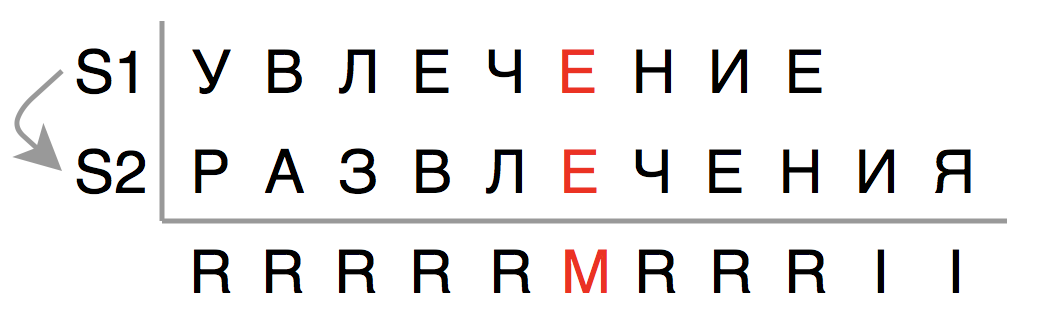
\includegraphics[scale=0.5]{ex1}}
	\textit{\caption{Пример нахождения расстояния Левенштейна}}
\end{figure}

\noindent Это не минимальное расстояние Левенштейна, следовательно существует проблема взаимного выравнивания строк. Более удачный вариант и зображен на рис. 2:

\clearpage

\vspace{\baselineskip}
\begin{figure}[h]
	\center{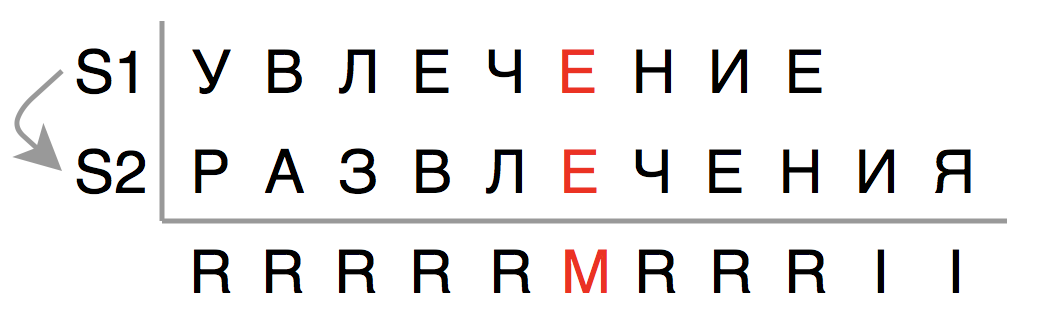
\includegraphics[scale=0.5]{ex1}}
	\textit{\caption{Пример эффективного нахождения расстояния Левенштейна}}
\end{figure}

\textbf{Математическая формулировка алгоритма}

Пусть даны 2 строки $S_1[1..i]$ и $S_2[1..j]$ длиной $i$ и $j$ соответственно. Расстояние в алгоритме Левенштейна можно посчитать с помощью рекурентной формулы:

\begin{equation*}
D(S_1[1..i],S_2[1..j]) =
\begin{cases}
	0,\text{ если }i=0,j=0
	\\
	i,\text{ если }j=0, i>0
	\\
	j,\text{ если }i=0, j>0
	\\
	min
	\begin{cases}
		D(S_1[1..i],S_2[1..j-1])+1\qquad\qquad\qquad\textit{	//I}
		\\
		D(S_1[1..i-1],S_2[1..j])+1\qquad\qquad\qquad\textit{    //D}
		\\
		D(S_1[1..i-1],S_2[1..j-1])+
		\\
		\left[
		\begin{gathered}
			0,\text{ если }S_1[i]==S_2[j],i>0,j>0\qquad\textit{//M}
			\\
			1,\text{ иначе}\qquad\qquad\qquad\qquad\qquad\qquad\quad\textit{     //R}
		\end{gathered}
		\right.
	\end{cases}
\end{cases}
\end{equation*}
где операции:
\begin{enumerate}
	\item вставка — I, штраф $=1$;
	\item замена — R, штраф $=1$;
	\item удаление — D, штраф $=1$;
	\item совпадение — M, штраф $=0$.
\end{enumerate}

\vspace{\baselineskip}

Можно описать поиск расстояния Левенштейна \underline{разными алгоритмами}:

\begin{enumerate}
	\item матричное рекурсивное расстояние;
	\item рекурсивный расчет по формуле \textit{(проблема - много лишних вычислений)};
	\item рекурсивный алгоритм, заполняющий незаполненные клетки матрицы \textit{(по аналогии с $\infty$ в алгоритме Дейкстры поиска расстояний в графе)}.
\end{enumerate}

\subsection{Расстояние Дамерау-Левенштейна}%

\textbf{Расстояние Дамерау-Левенштейна} включает также операцию перестановки двух соседних символов - \textit{транспозицию (Т)}.
\vspace{\baselineskip}

$D(\text{'}ab\text{'},\text{'}ba\text{'})=1$ — есть T

$D(\text{'}ab\text{'},\text{'}cd\text{'})$ — невозможна транспозиция

\vspace{\baselineskip}

Модификаця была введена, так как большинство ошибок пользователей при печати текста - банальные опечатки. Например, \textit{"аглоритм"} вместо \textit{"алгоритм"}.

\clearpage

\textbf{Математическая формулировка алгоритма}

Пусть даны 2 строки $S_1[1..i]$ и $S_2[1..j]$ длиной $i$ и $j$ соответственно.

\begin{equation*}
	D(S_1[1..i],S_2[1..j]) =
	\begin{cases}
	0,\text{ если }i=0,j=0
\\
i,\text{ если }j=0, i>0
\\
j,\text{ если }i=0, j>0
\\
		min
		\begin{cases}
			D(S_1[1..i],S_2[1..j-1])+1
			\\
			D(S_1[1..i-1],S_2[1..j])+1
			\\
			D(S_1[1..i-1],S_2[1..j-1])+
			\\
			\left[
			\begin{gathered}
				0,\text{ если }S_1[i]==S_2[j],i>0,j>0
				\\
				1,\text{ иначе}
			\end{gathered}
			\right.
			\\
			D(S_1[1..i-2],S_2[1..j-2])+1
		\end{cases},
	\text{ если }\begin{gathered}i>1,j>1,\\
		S_1[i]==S_2[j-1],\\
		S_1[j]==S_2[i-1]\end{gathered}
	\\min
			\begin{cases}
		D(S_1[1..i],S_2[1..j-1])+1
		\\
		D(S_1[1..i-1],S_2[1..j])+1
		\\
		D(S_1[1..i-1],S_2[1..j-1])+
		\\
		\left[
		\begin{gathered}
			0,\text{ если }S_1[i]==S_2[j],i>0,j>0
			\\
			1,\text{ иначе}
		\end{gathered}
		\right.
		\end{cases},
	\text{ иначе}
	\end{cases}
\end{equation*}
\vspace{\baselineskip}

\textbf{Вывод}

Были рассмотрены алгоритмы нахождения расстояния Левенштейна и его усовершенствованный алгоритм нахождения расстояния Дамерау-Левенштейна, принципиальная разница которого — наличие транспозиции, а также области применения данных алгоритмов.

\clearpage

% конс часть
\section{Конструкторская часть}%
\vspace{\baselineskip}

\subsection{Требования к программе}%

К программе предоставлены следующие требования:

\begin{enumerate}
	\item на ввод подается 2 строки;
	\item uppercase и lowercase буквы считаются разными;
	\item программа должна вывести расстояние и матрицу, если она использовалась;
	\item две пустые строки — корректный ввод, программа не должна аваийно завершаться.
\end{enumerate}

\subsection{Схемы алгоритмов}%

В данном разделе будут рассмотрены схемы следующих алгоритмов:
\begin{enumerate}
	\item матричного алгоритма нахождения расстояния Левенштейна (рис. 3);
	\item рекурсивного алгоритма нахождения расстояния Левенштейна (рис. 4);
	\item рекурсивного алгоритма нахождения расстояния Левенштейна с заполнением матрицы (рис. 5);
	\item матричного алгоритма нахождения расстояния Дамерау-Левенштейна (рис. 6);
	\item рекурсивного алгоритма нахождения расстояния Дамерау-Левенштейна (рис. 7).
\end{enumerate}

\begin{figure}[h]
	\center{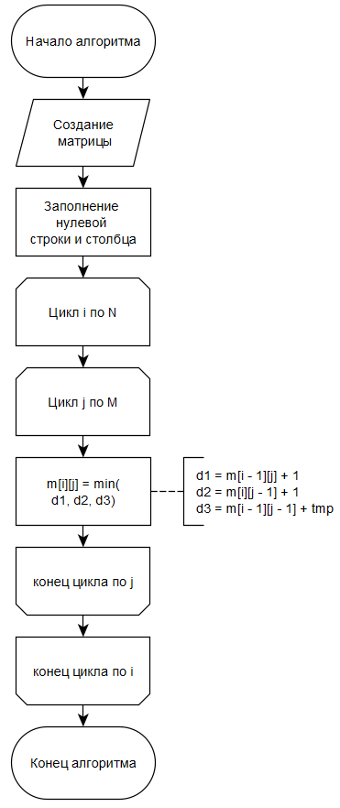
\includegraphics[scale=1.5]{alg1}}
	\textit{\caption{Схема матричного алгоритма нахождения расстояния Левенштейна}}
\end{figure}

\begin{figure}[h]
	\center{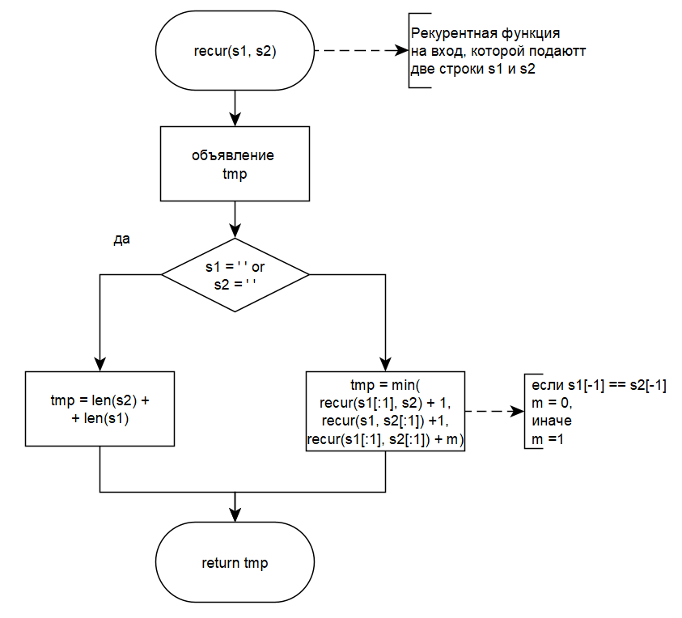
\includegraphics[scale=1.5]{alg2}}
	\textit{\caption{Схема рекурсивного алгоритма нахождения расстояния Левенштейна}}
\end{figure}

\begin{figure}[h]
	\centering
	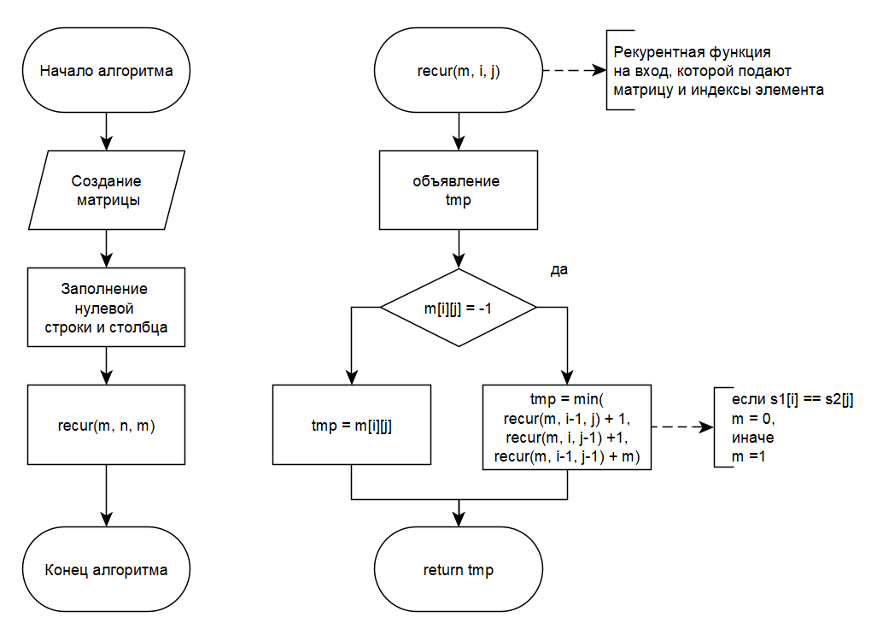
\includegraphics[scale=1.1]{alg3}
	\textit{\caption{Схема матрично-рекурсивного алгоритма нахождения расстояния Левенштейна}}
\end{figure}

\begin{figure}[h]
	\center{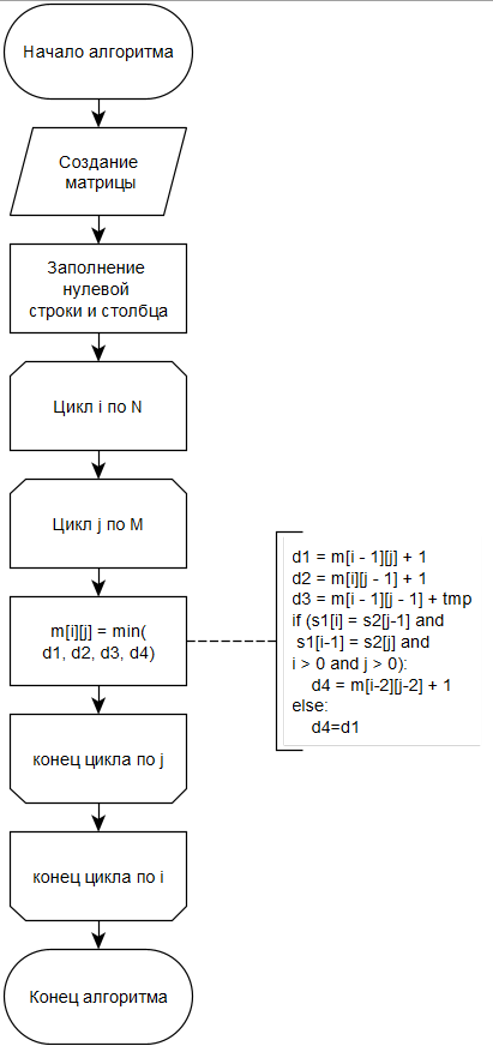
\includegraphics[scale=1.1]{alg4}}
	\textit{\caption{Cхема матричного алгоритма нахождения расстояния Дамерау-Левенштейна}}
\end{figure}

\begin{figure}[h]
	\center{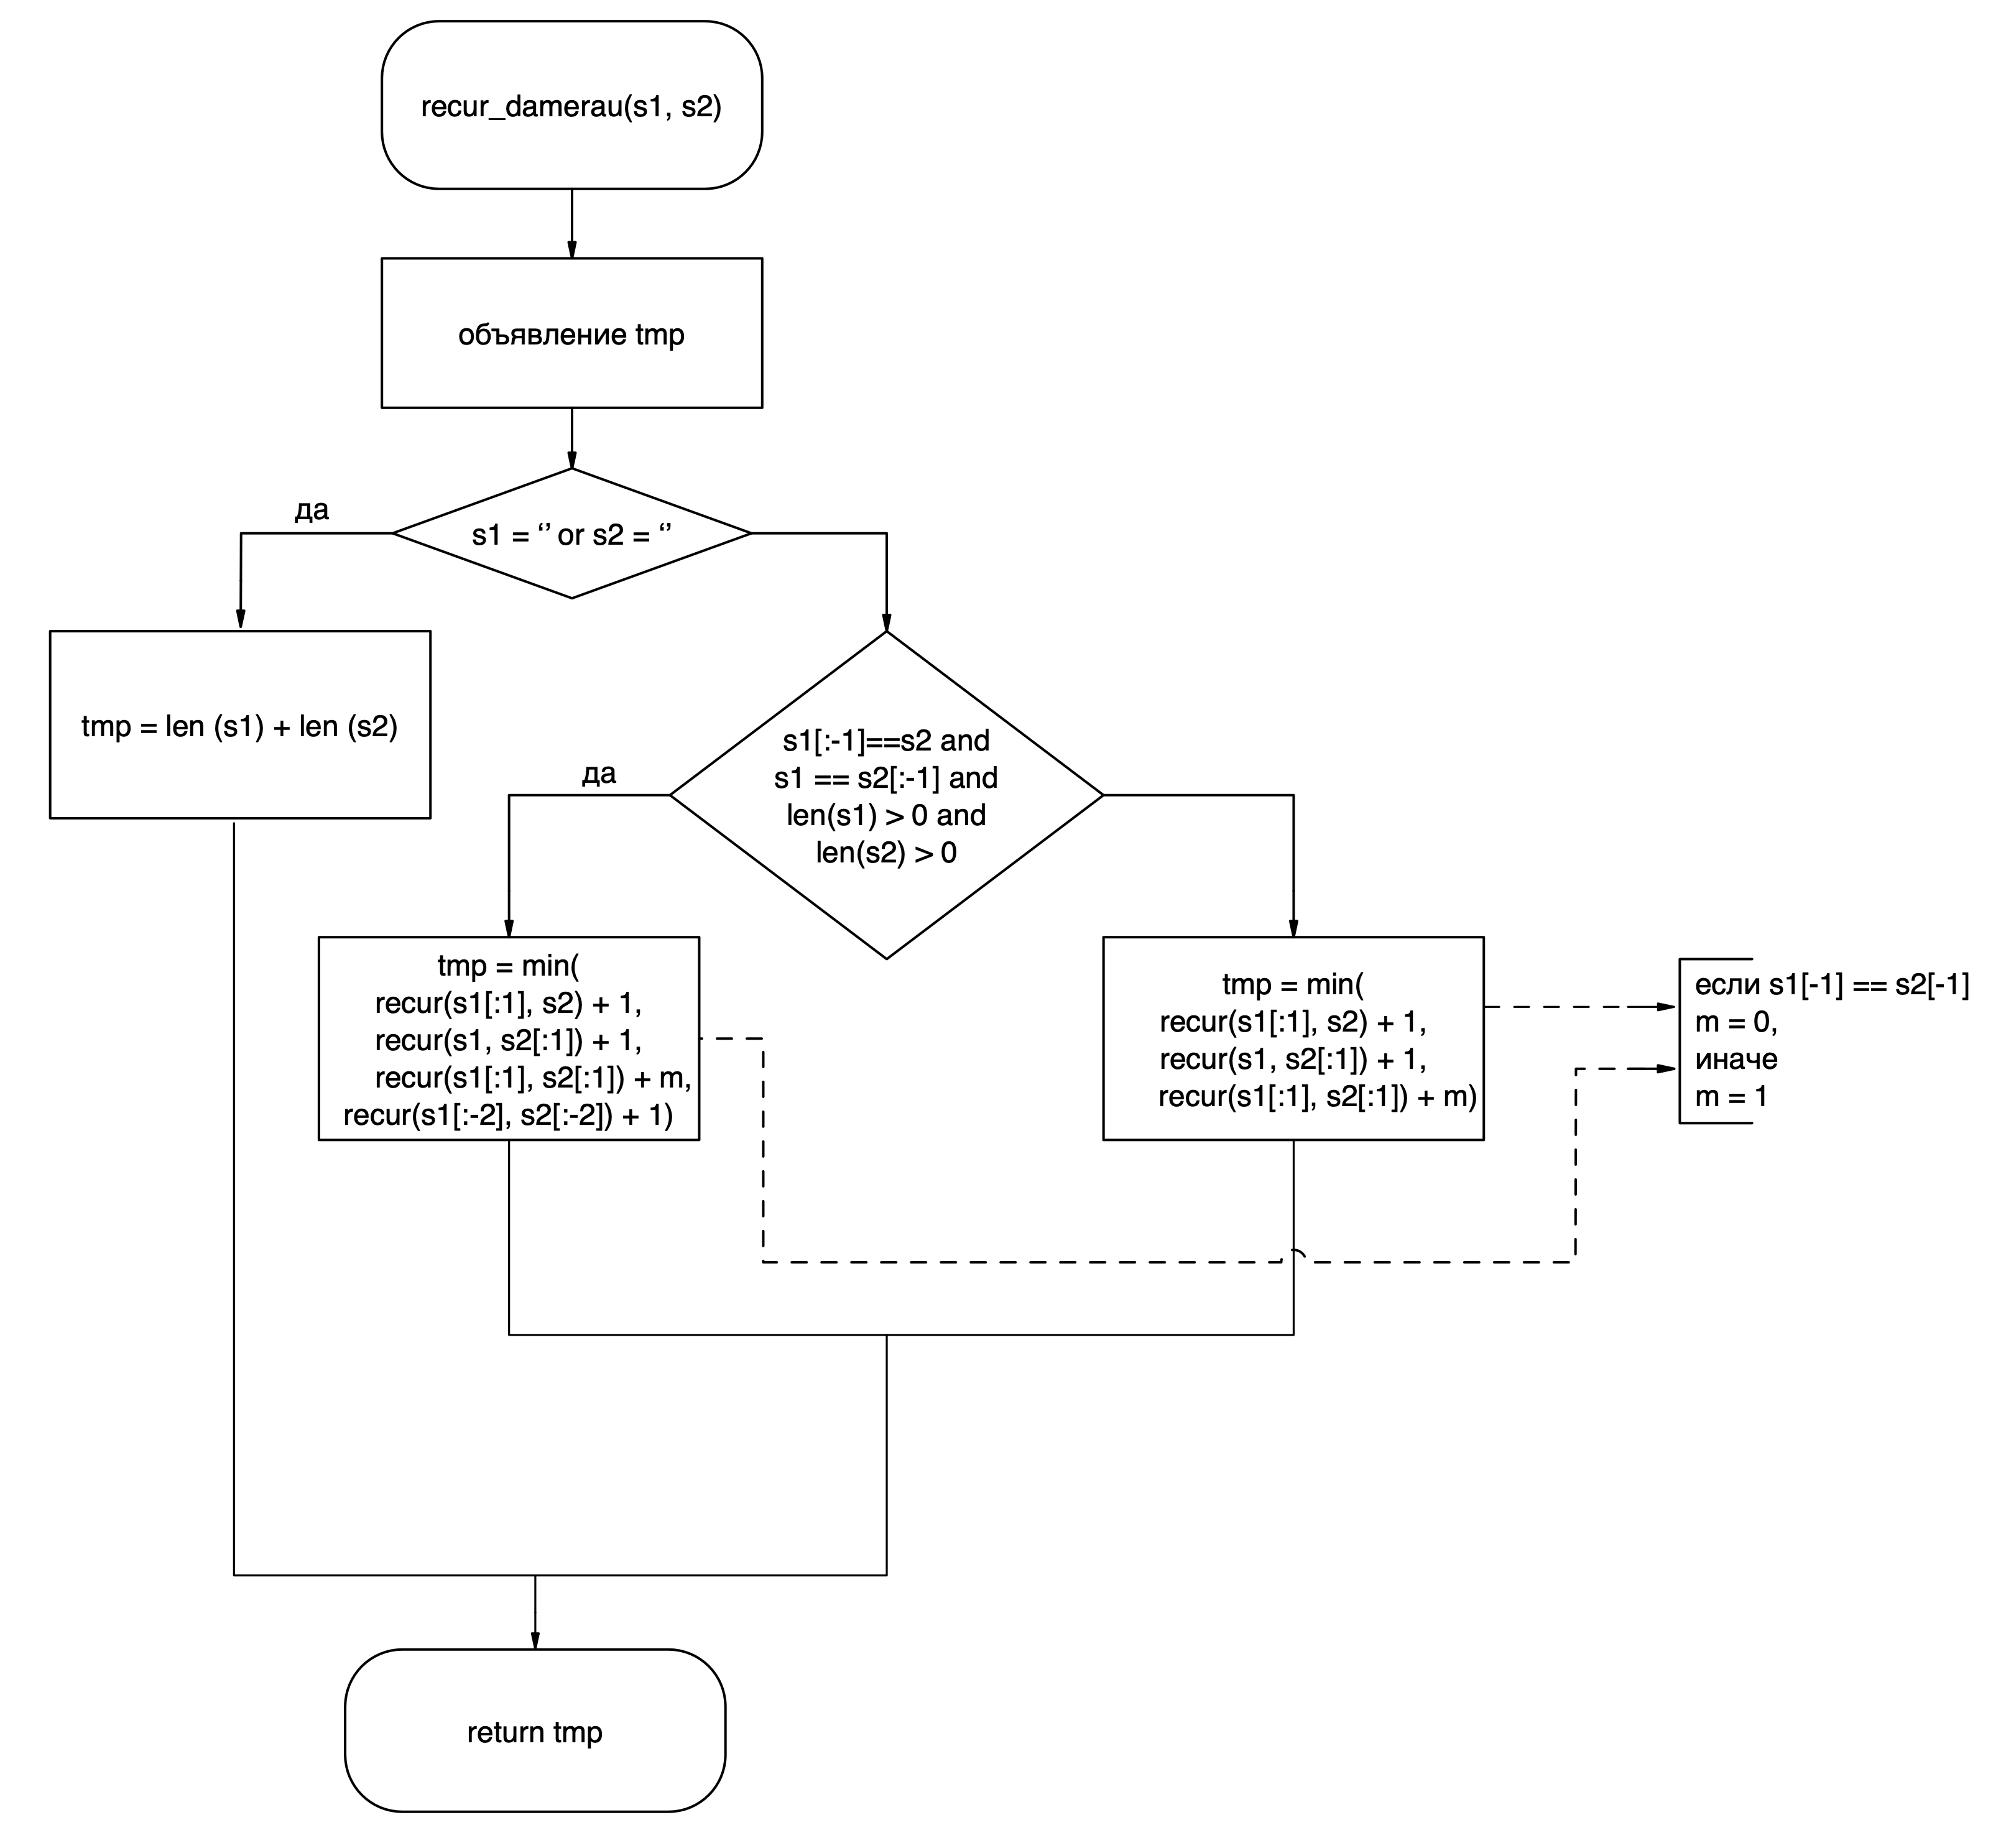
\includegraphics[scale=0.3]{alg5}}
	\textit{\caption{Cхема рекурсивного алгоритма нахождения расстояния Дамерау-Левенштейна}}
\end{figure}

\clearpage

\section{Технологическая часть}%
\vspace{\baselineskip}

\subsection{Выбор языка программирования}%

В качестве языка программирования был выбран python, т.к. данный язык программирования позволяет написать программу за короткое время. Для замера процессорного времени была использована функция 	process\symbol{95}time(), стандартной библиотеки python – time [2].

\subsection{Реализация алгоритмов}%

В листингах 1-5 представлена реализация алгоритмов нахождения расстояний Левенштейна и Дамерау-Левенштейна. 

В листинге 6 представлена функция для замера времени выполнения заданной функции на заданном количестве итераций на строках указанной длины.

\vspace{\baselineskip}

\noindent \textit{Листинг 1. Реализация алгоритма нахождения расстояния Левенштейна с заполнением матрицы.}

\begin{lstlisting}
def calc_dist_matrix(s1, s2):
	matr = np.eye(len(s1) + 1, len(s2) + 1)

	for i in range(len(s1) + 1):
		matr[i][0] = i
	for j in range(len(s2) + 1):
		matr[0][j] = j
	
	for i in range(len(s1)):
		for j in range(len(s2)):
			d1 = matr[i + 1][j] + 1
			d2 = matr[i][j + 1] + 1
			if s1[i] == s2[j]:
				d3 = matr[i][j]
			else:
				d3 = matr[i][j] + 1
			matr[i + 1][j + 1] = min(d1, d2, d3)
\end{lstlisting}

\noindent \textit{Листинг 2. Реализация рекурсивного алгоритма нахождения расстояния Левенштейна.}

\begin{lstlisting}
def calc_dist_recur(s1, s2, printable=False):
	if s1 == '' or s2 == '':
		return abs(len(s1) - len(s2))
	
	tmp = 0 if (s1[-1] == s2[-1]) else 1
	return min(calc_dist_recur(s1[:-1], s2) + 1,
					calc_dist_recur(s1, s2[:-1]) + 1,
					calc_dist_recur(s1[:-1], s2[:-1]) + tmp)
\end{lstlisting}

\clearpage

\noindent \textit{Листинг 3. Реализация рекурсивного алгоритма нахождения расстояния Левенштейна с заполнением матрицы.}

\begin{lstlisting}
def calc_dist_recur_matrix(s1, s2, printable=False):
	def calc_value(matr, i, j):
		if matr[i][j] != -1:
			return matr[i][j]
		else:
			tmp = 0 if (s1[i - 1] == s2[j - 1]) else 1
			matr[i][j] = min(calc_value(matr, i - 1, j) + 1,
									calc_value(matr, i, j - 1) + 1,
									calc_value(matr, i - 1, j - 1) + tmp)
			return matr[i][j]

	matr = np.full((len(s1) + 1, len(s2) + 1), -1)
	for i in range(len(s1) + 1):
		matr[i][0] = i
	for j in range(len(s2) + 1):
		matr[0][j] = j
	value = calc_value(matr, len(s1), len(s2))
\end{lstlisting}

\vspace{\baselineskip}

\noindent \textit{Листинг 4. Реализация алгоритма нахождения расстояния Дамерау-Левенштейна с заполнением матрицы.}

\begin{lstlisting}
def calc_dist_damerau(s1, s2):
	matr = np.eye(len(s1) + 1, len(s2) + 1)
	
	for i in range(len(s1) + 1):
		matr[i][0] = i
	for j in range(len(s2) + 1):
		matr[0][j] = j
	
	for i in range(len(s1)):
		for j in range(len(s2)):
			d1 = matr[i + 1][j] + 1
			d2 = matr[i][j + 1] + 1
			if s1[i] == s2[j]:
				d3 = matr[i][j]
			else:
				d3 = matr[i][j] + 1
			if s1[i] == s2[j - 1] and s1[i - 1] == s2[j] and i > 0 and j > 0:
				d4 = matr[i - 1][j - 1] + 1
			else:
				d4 = d1
			matr[i + 1][j + 1] = min(d1, d2, d3, d4)
\end{lstlisting}

\clearpage

\noindent \textit{Листинг 5. Реализация рекурсивного алгоритма нахождения расстояния Дамерау-Левенштейна.}

\begin{lstlisting}
def calc_dist_damerau_recur(s1, s2, printable=False):

	if s1 == '' or s2 == '':
		return abs(len(s1) - len(s2))

	tmp = 0 if (s1[-1] == s2[-1]) else 1
	if s1[:-1] == s2 and s1 == s2[:-1] and len(s1) > 0 and len(s2) > 0:
		return min(calc_dist_damerau_recur(s1[:-1], s2) + 1,
						calc_dist_damerau_recur(s1, s2[:-1]) + 1,
						calc_dist_damerau_recur(s1[:-1], s2[:-1]) + tmp,
						calc_dist_damerau_recur(s1[:-2], s2[:-2]) + 1)
	else:
		return min(calc_dist_damerau_recur(s1[:-1], s2) + 1,
						calc_dist_damerau_recur(s1, s2[:-1]) + 1,
						calc_dist_damerau_recur(s1[:-1], s2[:-1]) + tmp)

\end{lstlisting}

\noindent \textit{Листинг 6. Функция подсчета среднего времени выполнения программы для строк длиной length.}

\begin{lstlisting}
def time_analyze(function, iterations, length=5):
	t1 = process_time()
	for _ in range(iterations):
		s1 = random_string(length)
		s2 = random_string(length)
		function(s1, s2, False)
	
	t2 = process_time()
	return (t2 - t1) / iterations
\end{lstlisting}

\subsection{Тестирование функций}%

Для модульного тестирования реализованных алгоритмах (см. листинги 1-5) была использована стандартная библиотека языка python – unittest. Модульные тесты приведены в листингах 7-8. Все функции протестированы на пустые входящие строки, а также на различные другие входные данные. 

Для алгоритма поиска расстояния Дамерау-Левенштейна существует дополнительные отдельные тесты на транспозицию.

\vspace{\baselineskip}

\noindent \textit{Листинг 7. Проверка на пустоту строк}

\begin{lstlisting}
def test_empty(self):
	self.assertEqual(self.function('', ''), 0)
	self.assertEqual(self.function('a', ''), 1)
	self.assertEqual(self.function('', 'a'), 1)
\end{lstlisting}

\clearpage

\noindent \textit{Листинг 8. Проверка на выполнение операций}

\begin{lstlisting}
def test_different(self):
	# Match
	self.assertEqual(self.function('a', 'a'), 0)
	self.assertEqual(self.function('c', 'c'), 0)
	# Delete
	self.assertEqual(self.function('ab', 'a'), 1)
	self.assertEqual(self.function('op', 'o'), 1)
	# Insert
	self.assertEqual(self.function('a', 'ab'), 1)
	self.assertEqual(self.function('o', 'op'), 1)
	# Replace
	self.assertEqual(self.function('ab', 'aс'), 1)
	self.assertEqual(self.function('op', 'od'), 1)
\end{lstlisting}

\vspace{\baselineskip}

Все тесты пройдены успешно.

\clearpage

\section{Экспериментальная часть}%

При запуске программы первое, что видит пользователь, – это интуитивно понятный интерфейс.

\subsection{Интерфейс}%

На рис. 8 представлено главное меню программы. В зависимости от выбранного пункта меню запускается соответствующий алгоритм

\begin{center}
\begin{figure}[h]
	\center{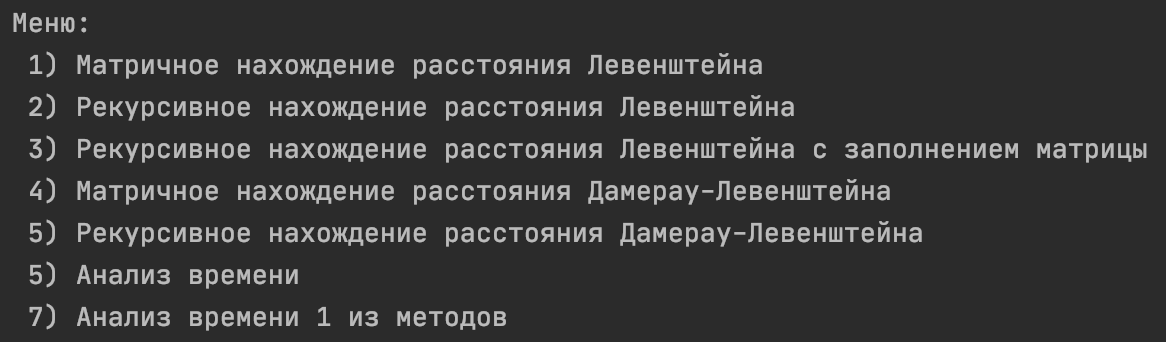
\includegraphics[scale=0.6]{scrin1}}
	\textit{\caption{Главное меню программы}}
\end{figure}
\end{center}

На рис. 9-12 приведены примеры работы программы при вводе строк \textit{«увлечение»} и \textit{«развлечения»} при выборе пунктов меню 1-5.

\begin{figure}[h]
	\center{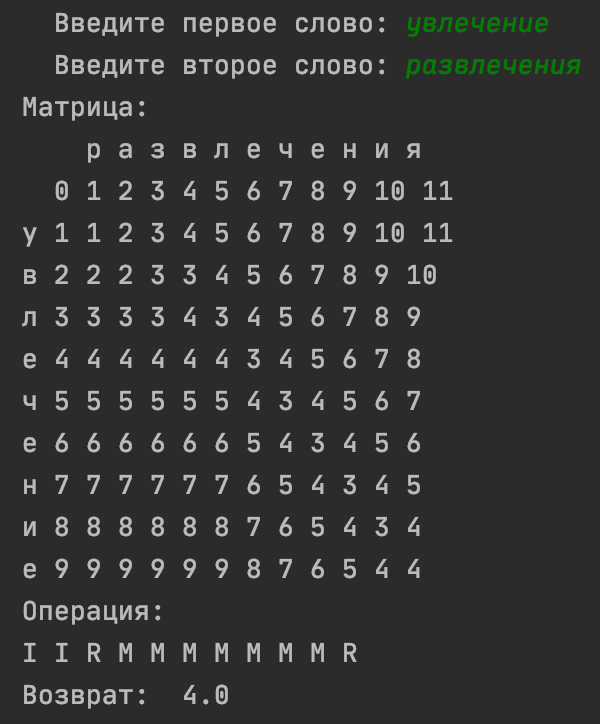
\includegraphics[scale=0.6]{scrin2}}
	\textit{\caption{Пример работы программы при выборе пункта 1}}
\end{figure}

\clearpage

\begin{figure}[h]
	\center{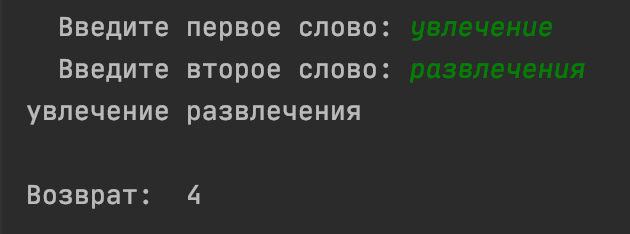
\includegraphics[scale=0.6]{scrin3}}
	\textit{\caption{Пример работы программы при выборе пункта 2}}
\end{figure}

\begin{figure}[h]
	\center{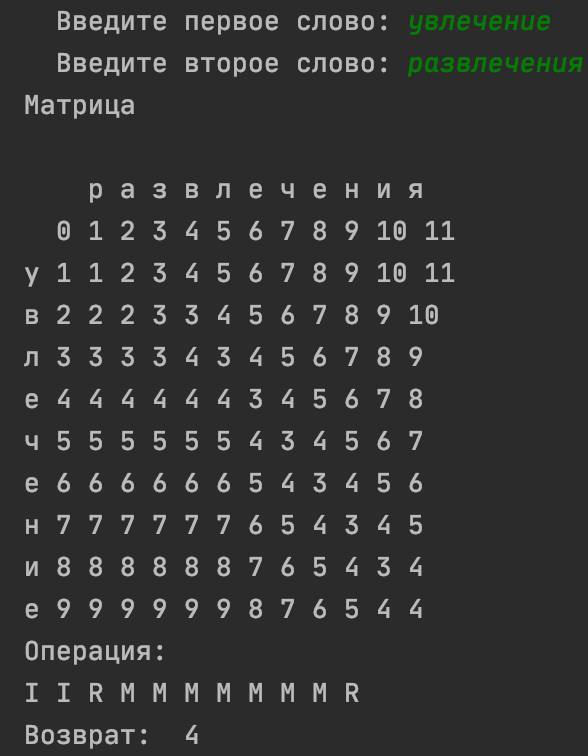
\includegraphics[scale=0.6]{scrin4}}
	\textit{\caption{Пример работы программы при выборе пункта 3}}
\end{figure}

\clearpage

\begin{figure}[h]
	\center{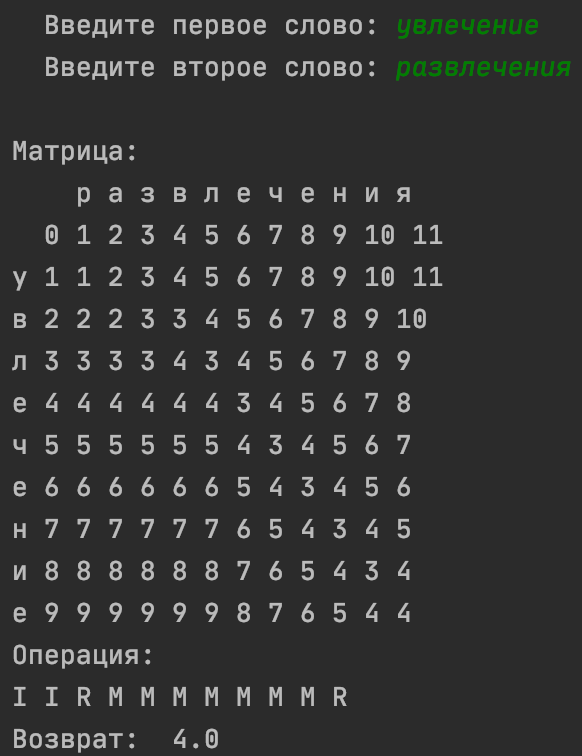
\includegraphics[scale=0.6]{scrin5}}
	\textit{\caption{Пример работы программы при выборе пункта 4}}
\end{figure}

\begin{figure}[h]
	\center{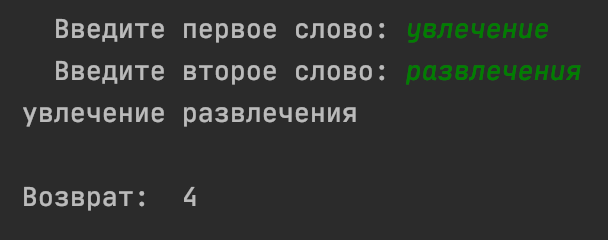
\includegraphics[scale=0.7]{scrin6}}
	\textit{\caption{Пример работы программы при выборе пункта 5}}
\end{figure}

\clearpage

\subsection{Сравнение алгоритмов по времени работы реализаций}%

Для сравнения в программе необходимо провести замеры процессорного времени для выполнения n – количества вычислений для строк одинаковой длины. Результаты замера времени предоставлены в таблице 1.

\begin{center}
	\textit{Таблица 1. Сравнение алгоритмов по времени}
\end{center}

\begin{tabular}{ | l | l | l | } \hline
	Алгоритм & Длина строк & Среднее время, сек  \\ \hline
	Левенштейн матричный & 5 & 0.00008750 \\
	Левенштейн матричный & 10 & 0.00029531 \\
	Левенштейн матричный & 15 & 0.00063480 \\
	Левенштейн рекурсивный & 5 & 0.00123438 \\
	Левенштейн рекурсивный & 7 & 0.03080775 \\
	Левенштейн рекурсивный & 10 & 5.73437500 \\
	Левенштейн рекурсивный с заполнением матрицы & 5  & 0.00012969 \\
	Левенштейн рекурсивный с заполнением матрицы & 10 & 0.00046875 \\
	Левенштейн рекурсивный с заполнением матрицы & 15 & 0.00098420 \\
	Дамерау-Левенштейн матричный & 5 & 0.00008906 \\
	Дамерау-Левенштейн матричный & 10 & 0.00032188 \\
	Дамерау-Левенштейн матричный & 15 & 0.00067355 \\ 
	Дамерау-Левенштейн рекурсивный & 5 & 0.00159060 \\
	Дамерау-Левенштейн рекурсивный & 7 & 0.03289530 \\
	Дамерау-Левенштейн рекурсивный & 10 & 5.47348705 \\ \hline
\end{tabular}

\vspace{\baselineskip}

Замеры времени усреднялись для каждого набора одинаковых экспериментов. Для этого все вычисления производились на случайных строках при 1000-10000 итераций, кроме рекурсивных, для которых количество итераций было в пределах 20-50, это связано с временем выполнения данных алгоритмов.

\vspace{\baselineskip}

\textbf{Вывод:} у матричных алгоритмов время пропорционально квадрату длины строк (при увеличении строки в два раза, время увеличивается в четыре раза). Рекурсивный алгоритм показывает наихудшее время, это связано с повторным вычислением одних и тех же значений (каждый вызов порождает три новых вызова, у которых могут дублироваться входные значения). Матричные алгоритмы по поиску расстояния Левенштейна и Дамерау-Левенштейна показывают самое лучшее время. Первый алгоритм немного быстрее, однако необходимо учитывать то, что второй решает другую задачу.

\subsection{Сравнение алгоритмов по затраченной памяти}%

Пусть длина строки S1 - n, длина строки S2 - m, тогда затраты памяти на приведенные выше алгоритмы будут следующими.

\vspace{\baselineskip}

Затраты памяти \textbf{матричного алгоритма нахождения расстояния Левенштейна}:\begin{enumerate}
	\item строки S1, S2 - (m + n) * sizeof(char);
	\item матрица - ((m + 1) * (n + 1)) * sizeof(int);
	\item длины строк - 2 * sizeof(int);
	\item вспомогательная переменная - sizeof(int).
\end{enumerate}

\vspace{\baselineskip}

Затраты памяти \textbf{рекурсивного алгоритма нахождения расстояния Левенштейна} (для каждого вызова):\begin{enumerate}
	\item строки S1, S2 - (m + n) * sizeof(char);
	\item длины строк - 2 * sizeof(int);
	\item вспомогательные переменные -  2 * sizeof(int);
	\item адрес возврата.
\end{enumerate}

\vspace{\baselineskip}

Затраты памяти рекурсивного алгоритма нахождения расстояния Левенштейна с заполнением матрицы:
\begin{enumerate}
	\item матрица - ((m + 1) * (n + 1)) * sizeof(int);
	\item строки S1, S2 - (m + n) * sizeof(char).
\end{enumerate}

\vspace{\baselineskip}

Для каждого рекурсивного вызова:
\begin{enumerate}
	\item передача данных - 2 * sizeof(int*) + sizeof(int**);
	\item вспомогательная переменная -  sizeof(int).
	\item адрес возврата
\end{enumerate}

\vspace{\baselineskip}

Чтобы получить итоговую оценку затрачиваемой памяти на рекурсивные вызовы необходимо затрачиваемую память для одного рекурсивного вызова умножить на максимальную глубину рекурсии, которая равна сложению длин входных строк.\vspace{\baselineskip}

\vspace{\baselineskip}

Затраты памяти \textbf{матричного алгоритма нахождения расстояния Дамерау-Левенштейна}:\begin{enumerate}
	\item строки S1, S2 - (m + n) * sizeof(char);
	\item матрица - ((m + 1) * (n + 1)) * sizeof(int);
	\item длины строк - 2 * sizeof(int);
	\item вспомогательная переменная  - sizeof(int).
\end{enumerate}

\vspace{\baselineskip}

Затраты памяти \textbf{рекурсивного алгоритма нахождения расстояния Дамерау-Левенштейна}:\begin{enumerate}
	\item строки S1, S2 - (m + n) * sizeof(char);
\item длины строк - 2 * sizeof(int);
\item вспомогательные переменные -  2 * sizeof(int);
\item адрес возврата.
\end{enumerate}

\vspace{\baselineskip}

Для каждого рекурсивного вызова:
\begin{enumerate}
	\item передача данных - 2 * sizeof(int*) + sizeof(int**);
	\item вспомогательная переменная -  sizeof(int).
	\item адрес возврата
\end{enumerate}

\vspace{\baselineskip}

\textbf{Вывод:} при большой длине строк, матричные методы занимают огромное количество памяти, в отличие от рекурсивного алгоритма. Сравнивая алгоритмы по затрачиваемой памяти, можно прийти к тому, что память для рекурсивного алгоритма зависит от n (длины строк) как $4*n2 + 164*n$, в то время, как память, необходимая для матричного алгоритма, – $(8 * n^2 + 2*n + 180)$, это говорит нам о том, что до n равного 31 включительно по памяти выигрывает матричный алгоритм, а начиная с длины строки 32 и более, рекурсивный алгоритм тратит меньше памяти, чем матричный.

\clearpage

\addcontentsline{toc}{section}{Заключение}

\section*{Заключение}

В ходе работы были изучены алгоритмы нахождения расстояний Левенштейна и Дамерау–Левенштейна. Реализованы 4 алгоритма поиска этих расстояний, приведен программный код реализации алгоритмов нахождения расстояний.

Было выполнено сравнение разных алгоритмов нахождения расстояния Левенштейна по затраченным ресурсам. Было установлено, что рекурсивный алгоритм занимает гораздо меньше памяти при работе со строками большой длины, чем матричные алгоритмы. Однако матричные алгоритмы отмечаются своим быстродействием. 

Цель работы достигнута. Алгоритмы нахождения расстояния Левенштейна и Дамерау-Левенштейна применены на практике, получены практические навыки реализации этих алгоритмов.

\clearpage

\addcontentsline{toc}{section}{Список литературы}

\section*{Список литературы}

[1] Вычисление расстояния Левенштейна // [Электронный ресурс]. Режим доступа: https://foxford.ru/wiki/informatika/vychislenie-rasstoyaniyalevenshteyna, свободный (дата обраще- ния: 06.09.21).

\vspace{\baselineskip}

[2] Официальный сайт Python, документация // [Электронный ресурс]. Режим доступа: https://docs.python.org/3/library/time.html, свободный (дата обращения: 06.09.21).

\end{document}